\documentclass[openany]{book}
\usepackage[utf8]{inputenc}
\usepackage[T1]{fontenc}
\usepackage{makecell}
\usepackage{float}
\usepackage[document]{ragged2e}
\usepackage[a4paper,top=2.54cm,bottom=2.54cm,left=2.54cm,right=2.54cm,marginparwidth=1.75cm]{geometry}
\usepackage{amsmath, amssymb}
\usepackage{graphicx}
\usepackage{colortbl} 
\usepackage{tikz}
\usepackage{subcaption}
\usepackage{amsfonts}
\setlength{\parindent}{.5 cm}   %Activar sangrias

\begin{document}

\begin{titlepage}
	\begin{center}
	\Huge{ UNIVERSIDAD DE GUADALAJARA\\}
	\vspace{.4 cm}
	\Huge{Centro Universitario de Ciencias Exactas\\
	e Ingenierías \\}
	\vspace{.4 cm}
	\LARGE{División de Ciencias Básicas\\}
	\LARGE{Licenciatura en Matemáticas\\}
	\vspace{1 cm}
	
\includegraphics[scale = .08]{escudo.png}\\
	\vspace{1 cm}
	\Large{Proyecto Integrador de Modelación Matemática\\}
	\vspace{1 cm}
	\LARGE{El transporte urbano de la Zona Metropolitana de Guadalajara desde la perspectiva de la teoría de grafos}\\
	\vspace{1 cm}
	{
	 	\large Fernando Betancourt Moreno\\
	}
	\vspace{1 cm}
	{
		\large Dr. Abel Palafox Gonzálex\\}   
		\end{center}
		\vspace{3.5 cm}
		\hfill{Guadalajara, Jal., Febrero 2025\\
	}
\end{titlepage}

\tableofcontents


\chapter{Introducción}

El transporte urbano en la Zona Metropolitana de Guadalajara (ZMG) es un componente fundamental para la movilidad de la población y el desarrollo económico de la región. A lo largo de las últimas décadas, la expansión de la mancha urbana ha avanzado de manera acelerada, promoviendo un crecimiento desordenado y fragmentado del territorio, lo que ha generado diversos retos en términos de movilidad e infraestructura (IMEPLAN, 2024). Este fenómeno ha resultado en una red de transporte público que enfrenta múltiples deficiencias, tales como la saturación en horas pico, tiempos de espera prolongados, falta de cobertura en zonas periféricas y una conectividad limitada entre distintos sistemas de transporte (IMEPLAN, 2024). Estas problemáticas afectan la calidad de vida de los habitantes y reducen la eficiencia de los desplazamientos dentro del área metropolitana.

El \textit{Plan de Ordenamiento Territorial Metropolitano del AMG (POTmet)} destaca la necesidad de implementar estrategias integrales que favorezcan la movilidad sustentable y permitan una mejor articulación del sistema de transporte público con el desarrollo urbano de la región (IMEPLAN, 2024). En este contexto, es esencial realizar estudios que permitan analizar la estructura actual de la red de transporte público con el objetivo de identificar áreas de mejora y proponer soluciones que optimicen su funcionamiento. La aplicación de herramientas analíticas basadas en modelos matemáticos puede contribuir significativamente a la toma de decisiones en materia de movilidad, proporcionando información cuantificable sobre la eficiencia de la red y sus niveles de accesibilidad.

Diversos estudios han abordado la movilidad en la ZMG desde distintas perspectivas, incluyendo encuestas de satisfacción de los usuarios, diagnósticos sobre cobertura y accesibilidad, así como planes de reestructuración de rutas. La \textit{Encuesta de Satisfacción a Usuarios del Transporte Público (2024)} señala que la percepción general del servicio es baja, con quejas recurrentes sobre la insuficiencia de rutas, la falta de puntualidad y la inseguridad en los trayectos (Polymetrix Consulting, 2024). Estos hallazgos reflejan la necesidad de analizar con mayor profundidad la estructura de la red y evaluar de manera objetiva su desempeño.

Dentro del \textit{POTmet}, se destaca la urgencia de fomentar un modelo de movilidad que promueva la intermodalidad, es decir, la combinación eficiente de distintos medios de transporte en un mismo desplazamiento, lo que permitiría reducir tiempos de viaje y mejorar la conectividad entre zonas clave de la metrópoli (IMEPLAN, 2024). Sin embargo, hasta el momento, los estudios sobre movilidad han privilegiado enfoques cualitativos o descriptivos, sin una aplicación sistemática de herramientas cuantitativas que permitan evaluar con precisión la conectividad de la red de transporte público.

Dado que el transporte público desempeña un papel clave en la movilidad urbana, resulta fundamental adoptar metodologías de análisis que permitan optimizar su funcionamiento. En este sentido, la teoría de grafos se presenta como una herramienta idónea para evaluar la eficiencia de la red de transporte mediante métricas que permiten identificar cuellos de botella, rutas críticas y oportunidades de mejora. Estudios recientes han demostrado la utilidad de la teoría de grafos para modelar matrices de origen-destino y evaluar la accesibilidad en redes multimodales, proporcionando una base cuantitativa para mejorar la planificación del transporte (Zhao et al., 2024; Barraza y Estrada, 2021).

Este estudio propone una nueva metodología basada en la teoría de grafos para analizar y optimizar la infraestructura del transporte público en la ZMG, promoviendo un esquema de movilidad más eficiente, accesible y equitativo. A través del uso de modelos matemáticos, se pretende analizar la estructura de la red de transporte y proponer intervenciones basadas en evidencia empírica que faciliten su modernización y mejora continua.

La pregunta de investigación que guía este trabajo es: \textit{¿Cómo puede la teoría de grafos proporcionar un enfoque metodológico para analizar la conectividad del sistema de transporte público en la ZMG?} A partir de esta interrogante, se pretende evaluar la conectividad del sistema de transporte, detectar posibles deficiencias estructurales y sugerir estrategias para optimizar su desempeño.

Para responder esta pregunta, se aplicará la teoría de grafos para modelar y analizar la red de transporte público en la ZMG. Se recopilarán datos sobre rutas, frecuencias y tiempos de traslado, representándolos en un \textit{grafo dirigido}. A partir de este modelo, se emplearán diversas métricas de análisis, tales como:

\begin{itemize}
	\item \textbf{Centralidad}: Para identificar las rutas y nodos más relevantes dentro de la red y evaluar su impacto en la conectividad global del sistema.
	\item \textbf{Conectividad}: Para analizar la accesibilidad de distintos puntos de la ciudad y medir la eficiencia de las conexiones entre diferentes rutas y modos de transporte.
	\item \textbf{Eficiencia}: Para examinar la relación entre tiempos de traslado, distancias recorridas y la optimización de la cobertura de la red.
	\item \textbf{Vulnerabilidad}: Para evaluar la resiliencia de la red ante la eliminación de nodos estratégicos y su impacto en la accesibilidad general (Barraza y Estrada, 2021).
\end{itemize}

Adicionalmente, se compararán estos resultados con modelos de planificación de transporte exitosos en otras ciudades, con el propósito de identificar buenas prácticas y adaptar soluciones que sean viables dentro del contexto de la ZMG.

Los objetivos de este estudio son los siguientes:

\textbf{Objetivo general:}
\begin{itemize}
	\item Evaluar la conectividad, accesibilidad y vulnerabilidad de la red de transporte público en la ZMG utilizando herramientas de teoría de grafos.
\end{itemize}

\textbf{Objetivos específicos:}
\begin{itemize}
	\item Identificar los nodos y rutas con mayor centralidad dentro de la red de transporte público.
	\item Analizar la eficiencia y accesibilidad del sistema en términos de tiempos de traslado y cobertura.
	\item Evaluar la vulnerabilidad del sistema ante la eliminación de nodos críticos y su impacto en la conectividad.
	\item Comparar los resultados con modelos de planificación en otras ciudades y proponer mejoras para la ZMG.
\end{itemize}

\textbf{Hipótesis:}
\begin{itemize}
	\item La aplicación de la teoría de grafos permitirá desarrollar y validar un enfoque metodológico cuantitativo para analizar la conectividad de la red de transporte público de la ZMG, proporcionando un marco analítico para futuras estrategias de optimización del sistema.
\end{itemize}

\textbf{Limitaciones:} Si bien el presente estudio aporta un marco metodológico innovador basado en la teoría de grafos para analizar la conectividad del sistema de transporte público en la ZMG, es importante reconocer algunas limitaciones inherentes. En primer lugar, la falta de datos de alta calidad sobre los orígenes y destinos limita la precisión en la estimación de los flujos de pasajeros. Además, el modelo no discrimina entre los diferentes tipos de transporte ni considera las variaciones en el aforo que cada uno soporta, asumiendo una homogeneidad que simplifica la realidad operativa. Finalmente, se ha supuesto que los horarios se cumplen a la perfección, sin contemplar la posibilidad de retrasos u otras variabilidades operativas. Estas limitaciones abren la puerta a futuras investigaciones que integren fuentes de datos complementarias y aborden la heterogeneidad y la incertidumbre en la operación del sistema.

\textbf{Estructura del documento:}
El documento está organizado en cinco capítulos. En el Capítulo 2 se presenta el marco teórico, abordando estudios previos y fundamentos de la teoría de grafos en el análisis de transporte. El Capítulo 3 describe la metodología empleada, detallando la recolección y procesamiento de datos. En el Capítulo 4 se presentan los resultados del análisis y su discusión. Finalmente, en el Capítulo 5 se exponen las conclusiones y recomendaciones para futuras investigaciones.

\chapter{Marco Teórico}
	\section{Fundamentos de la teoría de grafos}
	
		\subsection{Definición y conceptos básicos}

			Un \textbf{grafo} $G$ es una estructura matemática definida como un par ordenado:
			\begin{equation}
				G = (V, E)
			\end{equation}
			donde:
			\begin{itemize}
				\item $V$ es un conjunto no vacío de elementos llamados \textbf{vértices} o \textbf{nodos}.
				\item $E$ es un subconjunto de $V \times V$, cuyos elementos se denominan \textbf{aristas}.
			\end{itemize}
			
				\subsubsection{Tipos de grafos}
				
				Dependiendo de las propiedades de $E$, los grafos pueden clasificarse en diversas categorías:
				
				\begin{itemize}
					\item \textbf{Grafo no dirigido}: Un grafo es no dirigido si las aristas no tienen una orientación específica, es decir, $(u, v) \in E$ implica que $(v, u) \in E$.
					
						\begin{center}
							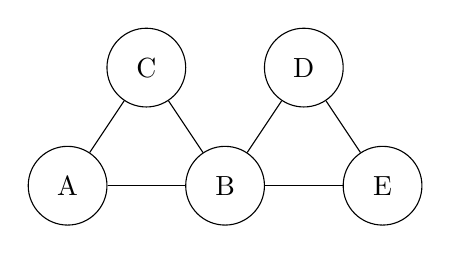
\begin{tikzpicture}[scale=1, every node/.style={draw, circle, minimum size=1cm}]
								\node (A) at (0,0) {A};
								\node (B) at (2,0) {B};
								\node (C) at (1,1.5) {C};
								\node (D) at (3,1.5) {D};
								\node (E) at (4,0) {E};
								
								\draw (A) -- (B);
								\draw (A) -- (C);
								\draw (B) -- (C);
								\draw (B) -- (D);
								\draw (B) -- (E);
								\draw (D) -- (E);
							\end{tikzpicture}
						\end{center}
					
					\item \textbf{Grafo dirigido (dígrafo)}: En un grafo dirigido, cada arista tiene una dirección, por lo que $(u, v) \in E$ no implica necesariamente que $(v, u) \in E$ pero tampoco lo prohíbe. Dado este escenario, diremos que \textbf{$u$ se dirige a $v$}.
					
						\begin{center}
							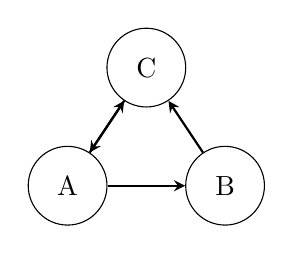
\begin{tikzpicture}[scale=1, every node/.style={draw, circle, minimum size=1cm}, >=stealth]
								\node (A) at (0,0) {A};
								\node (B) at (2,0) {B};
								\node (C) at (1,1.5) {C};
								
								\draw[->, thick] (A) -- (B);
								\draw[->, thick] (B) -- (C);
								\draw[->, thick] (C) -- (A);
								\draw[->, thick] (A) -- (C);
							\end{tikzpicture}
						\end{center}
					\item \textbf{Grafo ponderado}: Un grafo es ponderado si a cada arista $(u, v) \in E$ se le asigna un peso $w(u, v) \in \mathbb{R}$ que representa costos, distancias, o cualquier otra métrica relevante. Un grafo puede ser ponderado a la vez que dirigido o no dirigido.
					    \begin{center}
						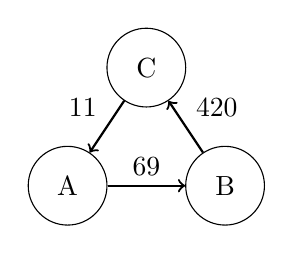
\begin{tikzpicture}[scale=1, 
							vertex/.style={draw, circle, minimum size=1cm}
							]
							% Definición de vértices
							\node[vertex] (A) at (0,0) {A};
							\node[vertex] (B) at (2,0) {B};
							\node[vertex] (C) at (1,1.5) {C};
							
							% Aristas con etiquetas; se anula el estilo global para estos nodos
							\draw[->, thick] (A) -- node[above, draw=none, fill=none] {69} (B);
							\draw[->, thick] (B) -- node[above right, draw=none, fill=none] {420} (C);
							\draw[->, thick] (C) -- node[above left, draw=none, fill=none] {11} (A);
						\end{tikzpicture}
					\end{center}
	
				\end{itemize}
							
			En delante nos ocuparemos únicamente de los grafos dirigidos sean ponderados o no y, por simplicidad, asumiremos que no existen vértices que se dirijan a sí mismos. Es decir, $(v, v) \notin E$ para ningún $v \in V$.

		
		\subsection{Propiedades fundamentales de los grafos}
			Los grafos poseen diversas propiedades matemáticas que permiten su análisis estructural.
			Algunas que son especialmente valiosas para el presente estudio son conceptos como la \textit{conectividad}, que nos permite mesurar la importancia que tiene un nodo con respecto a los demás; así también los \textit{caminos}, que nos permiten representar trayectorias; entre otros conceptos.
			
			\subsubsection{Subgrafos}
			
			Un subgrafo $H = (V_H, E_H)$ de un grafo $G = (V, E)$ es un grafo tal que $V_H \subseteq V$ y $E_H \subseteq E$.
			Es decir, un subgrafo es una parte de un grafo que mantiene la estructura de nodos y aristas del grafo original.
			
			Muchos conceptos en la teoría de grafos pueden describirse en términos de subgrafos.
			
			\subsubsection{Caminos}
			
			Un \textbf{camino} en un grafo $G$ es un subgrafo en el que los vértices están conectados por una secuencia de aristas sin repeticiones:
			\begin{equation}
				P_k = (v_1, v_2, \dots, v_k) \quad \text{donde } \{v_i, v_{i+1}\} \in E, \forall i \in \{1, \dots, k-1\}.
			\end{equation}
			
			Los caminos son fundamentales en redes, pues permiten analizar rutas eficientes y la conectividad entre distintos puntos.
			
			\subsubsection{Ciclos}
			
			Un \textbf{ciclo} es un camino en el que el primer y el último vértice son el mismo:
			\begin{equation}
				C_k = (v_1, v_2, \dots, v_k, v_1) \quad \text{donde } \{v_k, v_1\} \in E.
			\end{equation}
			
			Los ciclos en redes ayudan a identificar redundancias estructurales y evaluar posibles congestiones en ciertas áreas.
			
			\begin{figure}[ht]
				\centering
				\begin{subfigure}{0.3\textwidth}
					\centering
					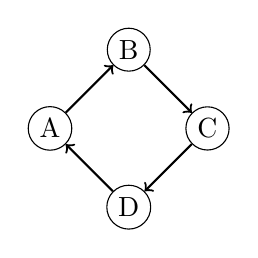
\begin{tikzpicture}[scale=1, every node/.style={circle, draw, fill=white, inner sep=2pt}]
						\node (a) at (0,0) {A};
						\node (b) at (1,1) {B};
						\node (c) at (2,0) {C};
						\node (d) at (1,-1) {D};
						\draw[->, thick] (a) -> (b);
						\draw[->, thick] (b) -> (c);
						\draw[->, thick] (c) -> (d);
						\draw[->, thick] (d) -> (a);
					\end{tikzpicture}
					\caption{Subgrafo}
				\end{subfigure}
				\begin{subfigure}{0.3\textwidth}
					\centering
					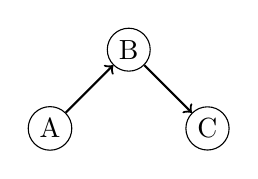
\begin{tikzpicture}[scale=1, every node/.style={circle, draw, fill=white, inner sep=2pt}]
						\node (a) at (0,0) {A};
						\node (b) at (1,1) {B};
						\node (c) at (2,0) {C};
						\draw[->, thick] (a) -> (b);
						\draw[->, thick] (b) -> (c);
					\end{tikzpicture}
					\caption{Camino}
				\end{subfigure}
				\begin{subfigure}{0.3\textwidth}
					\centering
					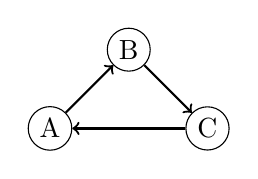
\begin{tikzpicture}[scale=1, every node/.style={circle, draw, fill=white, inner sep=2pt}]
						\node (a) at (0,0) {A};
						\node (b) at (1,1) {B};
						\node (c) at (2,0) {C};
						\draw[->, thick] (a) -> (b);
						\draw[->, thick] (b) -> (c);
						\draw[->, thick] (c) -> (a);
					\end{tikzpicture}
					\caption{Ciclo}
				\end{subfigure}
				\caption{Ejemplos de subgrafo, camino y ciclo en un grafo.}
			\end{figure}

			\subsubsection{Matriz de Adyacencia}
				La matriz de adyacencia es una representación matricial que codifica la estructura de un grafo. Dado un grafo $G=(V,E)$ con $N$ nodos, se define una matriz $A \in \mathbb{R}^{N \times N}$, donde cada elemento $a_{ij}$ indica si existe una conexión directa entre el nodo $i$ y el nodo $j$. En un grafo no ponderado, se establece que:
				\begin{equation}
					a_{ij} =
					\begin{cases}
						1, & \text{si existe una arista entre } i \text{ y } j,\\
						0, & \text{en caso contrario.}
					\end{cases}
				\end{equation}
				En grafos ponderados, cada $a_{ij}$ toma el valor del peso asignado a la conexión, lo que permite cuantificar la intensidad o costo de dicha relación.


		
		\subsection{Métricas clave en teoría de grafos}
		
			Las métricas en teoría de grafos permiten cuantificar diversas propiedades estructurales de un grafo y son esenciales para evaluar redes de transporte urbano. A continuación, se presentan algunas de las métricas más relevantes.
			
			\subsubsection{Grado de un Nodo}
			El grado de un nodo $v$, denotado como $deg(v)$, es el número de aristas incidentes a $v$. En un grafo dirigido, se distinguen el grado de entrada $deg^-(v)$ y el grado de salida $deg^+(v)$:
			\begin{align}
				deg^-(v) &= |\{ u \in V : (u,v) \in E \}|, \\
				deg^+(v) &= |\{ u \in V : (v,u) \in E \}|.
			\end{align}
			
			\subsubsection{Distancia entre Nodos}
			La distancia entre dos nodos $u$ y $v$, denotada como $d(u,v)$, es la longitud del camino más corto entre ellos, es decir, el número mínimo de aristas que deben recorrerse para ir de $u$ a $v$.
			\begin{equation}
				d(u,v) = \min \{ k \mid \exists (u = v_0, v_1, \dots, v_k = v) \text{ tal que } (v_i, v_{i+1}) \in E, \forall i \}.
			\end{equation}
			Si no existe un camino entre $u$ y $v$, se define $d(u,v) = \infty$.
			
			\subsubsection{Centralidad}
			La centralidad mide la importancia relativa de un nodo en un grafo. Existen diversas formas de centralidad:
			\begin{itemize}
				\item \textbf{Centralidad de grado}: Se define por el grado de un nodo, reflejando su conectividad local.
				\item \textbf{Centralidad de cercanía}: Se basa en la inversa de la suma de las distancias a todos los demás nodos:
				\begin{equation}
					C_c(v) = \frac{1}{\sum_{u \in V} d(v,u)}.
				\end{equation}
				\item \textbf{Centralidad de intermediación}: Representa cuántos caminos más cortos pasan por un nodo:
				\begin{equation}
					C_b(v) = \sum_{s \neq v \neq t} \frac{\sigma_{st}(v)}{\sigma_{st}},
				\end{equation}
				donde $\sigma_{st}$ es el número de caminos más cortos entre $s$ y $t$, y $\sigma_{st}(v)$ es el número de esos caminos que pasan por $v$.
			\end{itemize}
			
			\subsubsection{Densidad del Grafo}
			La densidad de un grafo mide qué tan conectado está en comparación con el máximo posible:
			\begin{equation}
				D = \frac{|E|}{|V|(|V|-1)}.
			\end{equation}

			\subsubsection{Vulnerabilidad}
			La \emph{vulnerabilidad} de un grafo se refiere a la sensibilidad de su estructura ante la eliminación de ciertos nodos.
			Sea $G$ un grafo de $N$ nodos y sea $E(G)$ la eficiencia global del grafo, definida como
			\begin{equation}
				E(G) = \frac{1}{N(N-1)} \sum_{\substack{i,j \\ i \neq j}} \frac{1}{d_{ij}},
			\end{equation}
			donde $d_{ij}$ representa la longitud de la trayectoria más corta entre los nodos $i$ y $j$. Si se elimina un conjunto $H$ de nodos críticos, se obtiene el grafo $G \setminus H$ con eficiencia $E(G \setminus H)$.
			La vulnerabilidad $V$ se expresa de la siguiente manera:
			\begin{equation}
			V = \frac{E(G) - E(G \setminus H)}{E(G)}.
			\end{equation}
			Un valor elevado de $V$ indica que la eliminación de los nodos críticos reduce significativamente la eficiencia global del grafo.

			\subsubsection{Largo Promedio por Camino}
			El \emph{largo promedio por camino} es una medida que cuantifica la distancia media entre todos los pares de nodos en un grafo. Se calcula mediante la siguiente expresión:
			\begin{equation}
				L = \frac{1}{N(N-1)} \sum_{\substack{i,j \\ i \neq j}} d_{ij},
			\end{equation}
			donde $N$ es el número total de nodos y $d_{ij}$ representa la longitud del camino más corto entre los nodos $i$ y $j$. Un valor menor de $L$ indica que, en promedio, los nodos están más próximos, lo cual se asocia con una mayor eficiencia en la conectividad del grafo.

			\subsubsection{Brecha Espectral (Gap Espectral)}
			La \emph{brecha espectral} es una medida derivada del espectro del grafo que refleja la diferencia entre los autovalores más importantes de un operador asociado al grafo, como la matriz de adyacencia. Si denotamos por $\lambda_1 \geq \lambda_2 \geq \cdots \geq \lambda_N$ a los autovalores de la matriz de adyacencia, la brecha espectral se define como:
			\begin{equation}
				\Delta = \lambda_1 - \lambda_2.
			\end{equation}
			Un valor mayor de $\Delta$ sugiere que el grafo posee una estructura más cohesiva y es menos vulnerable a desconexiones, ya que una diferencia significativa entre el primer y el segundo autovalor indica una robusta conectividad estructural.

		\subsection{Algoritmos fundamentales en teoría de grafos}
			Los algoritmos en teoría de grafos permiten resolver problemas fundamentales como la determinación de caminos más cortos entre nodos. En esta sección, se presentan dos algoritmos esenciales para este propósito: Dijkstra y Floyd-Warshall.

			\subsubsection{Algoritmo de Dijkstra}

			El algoritmo de Dijkstra encuentra el camino más corto desde un nodo fuente $s$ hacia todos los demás nodos en un grafo ponderado con pesos no negativos. Se basa en una estrategia voraz que mantiene un conjunto de nodos visitados y actualiza iterativamente las distancias más cortas conocidas.

			\textbf{Entrada:}
			\begin{itemize}
				\item Un grafo dirigido o no dirigido $G = (V, E)$ con pesos no negativos $w: E \to \mathbb{R}^+$.
				\item Un nodo fuente $s \in V$.
			\end{itemize}

			\textbf{Salida:}
			\begin{itemize}
				\item Distancias mínimas $d(v)$ desde $s$ hacia cada nodo $v \in V$.
				\item Árbol de caminos más cortos.
			\end{itemize}

			\textbf{Procedimiento:}
			\begin{enumerate}
				\item Inicializar $d(s) = 0$ y $d(v) = \infty$ para todos los $v \neq s$.
				\item Crear un conjunto de nodos visitados $S = \emptyset$.
				\item Mientras $S \neq V$:
				\begin{enumerate}
					\item Seleccionar el nodo $u \notin S$ con la menor distancia $d(u)$.
					\item Agregar $u$ a $S$.
					\item Para cada vecino $v$ de $u$ tal que $(u,v) \in E$:
					\begin{itemize}
						\item Si $d(u) + w(u,v) < d(v)$, actualizar $d(v) = d(u) + w(u,v)$.
					\end{itemize}
				\end{enumerate}
			\end{enumerate}

			\subsubsection{Algoritmo de Floyd-Warshall}

			El algoritmo de Floyd-Warshall encuentra el camino más corto entre todos los pares de nodos en un grafo ponderado con pesos arbitrarios (incluyendo negativoss). Se basa en la programación dinámica y mejora iterativamente una matriz de distancias.

			\textbf{Entrada:}
			\begin{itemize}
				\item Un grafo dirigido $G = (V, E)$ con una matriz de pesos $W$.
			\end{itemize}

			\textbf{Salida:}
			\begin{itemize}
				\item Una matriz $D$ donde $D[i][j]$ representa la distancia más corta entre los nodos $i$ y $j$.
			\end{itemize}

			\textbf{Procedimiento:}
			\begin{enumerate}
				\item Inicializar $D$ como la matriz de adyacencia $W$, donde $D[i][j] = w(i,j)$ si existe una arista $(i,j)$, y $\infty$ en caso contrario.
				\item Para cada nodo intermedio $k \in V$:
				\begin{enumerate}
					\item Para cada par de nodos $i, j \in V$:
					\begin{itemize}
						\item Si $D[i][k] + D[k][j] < D[i][j]$, actualizar $D[i][j] = D[i][k] + D[k][j]$.
					\end{itemize}
				\end{enumerate}
			\end{enumerate}

	\section{División territorial de la ZMG}
		La ZMG cuenta con un organismo llamado \textit{imeplan}, dedicado a "diseñar, gestionar e impulsar herramientas para el crecimiento integral de la ciudad desde un enfoque sustentable y resiliente" (imeplan, 2023). Este organismo publicó en 2016 el documento \textit{POTmet: plan de ordenamiento territorial metropolitano del AMG} (POTmet, en delante). Dentro de dicho documento el imeplan propone una forma de segmentar a la ZMG basándose en un modelo policéntrico de ciudad que "busca a través de una identificación metódica de las centralidades, contribuir a un mejor equilibrio espacial en el territorio del AMG, mejorando la distribución de equipamiento, la repartición de la población, la administración de las zonas para crecimiento y en general, todo lo que contribuya a fortalecer un sistema de ciudades aún incipiente en el territorio metropolitano" (imeplan, 2016, p. 265). Dichas centralidades permiten una mejor planificación y análisis de la movilidad urbana, facilitando el diseño de estrategias de transporte más eficientes (imeplan, 2016).

			\subsubsection{Definición y delimitación de la ZMG}
				La ZMG está conformada por los municipios de Guadalajara, Zapopan, Tlaquepaque, Tonalá, El Salto, Ixtlahuacán de los Membrillos y Juanacatlán.
				Su delimitación geográfica se encuentra establecida en el Plan de Ordenamiento Territorial Metropolitano (imeplan, 2016).

			\subsubsection{Centralidades}
				En el POTmet se define centralidad de la siguiente manera:
				\begin{center}
					Son unidades urbanas vinculadas por una estructura vial y que desempeñan una función esencial en la dinámica urbana del área metropolitana, definidas esencialmente por su concentración de empleo, población, transporte y prestación de servicios, además se caracterizan por un alto potencial de generación de identidad y arraigo entre sus habitantes.
				\end{center}
				Para delimitar estas centralidades se toman en cuenta aquellas concentraciones urbanas de entre 10,000 y 500,000 habitantes (imeplan, 2016), luego se estiman los siguientes métricos para cada una de ellas:

				\begin{itemize}
					\item \textbf{Productividad}
					\begin{itemize}
						\item Unidades económicas: cantidad de unidades económicas por centralidad.
						\item Personal ocupado: personal ocupado generado por las unidades económicas.
						\item Índice de demanda laboral (promedio): describe la relación entre población residente local y oferta laboral local.
						\item Densidad de población residente: Capas de datos que contienen los valores de densidad de población (personas/ha) por manzanas de la ZMG.
					\end{itemize}

					\item \textbf{Infraestructura}
					\begin{itemize}
						\item Rutas de transporte público: Cantidad de rutas que interceptan con la centralidad.
						\item Capacidad de carga de transporte público: Definida a través del cálculo de flota entre intervalo de las rutas de transporte público que interceptan con la centralidad.
						\item Transporte público masivo: Cantidad de líneas de transporte público masivo que interceptan por centralidad.
					\end{itemize}

					\item \textbf{Calidad de vida}
					\begin{itemize}
						\item Índice de suficiencia de servicios (promedio).
						\item Equipamientos distritales: Proporcionados por los municipios en sus PPDU y clasificados con base en el reglamento estatal de zonificación. Son polígonos de equipamiento de educación, cultura, salud, servicios institucionales y culto que sirven a amplios sectores de los centros de población.
						\item Equipamientos centrales: Proporcionados por los municipios en sus PPDU y clasificados con base en el reglamento estatal de zonificación. Son polígonos de equipamiento que sirven a la totalidad del centro de población.
						\item Equipamientos regionales: Proporcionados por los municipios en sus PPDU y clasificados con base en el reglamento estatal de zonificación. Son polígonos de equipamiento con cobertura de servicio que supera a la ciudad.
					\end{itemize}

					\item \textbf{Otros indicadores}
					\begin{itemize}
						\item Ponderación: Peso relativo de cada centralidad en la evaluación global.
					\end{itemize}
				\end{itemize}

			Una vez se obtienen estas métricas, los datos se normalizan y se otorga un peso a cada centralidad tomando como referencia a la centralidad que mayor puntaje haya obtenido. De este proceso obtenemos la siguiente tabla:

			\begin{table}[H]
			\centering
			\scriptsize
			\setlength{\tabcolsep}{3pt}
			\begin{tabular}{|l|c|c|c|c|c|c|c|c|c|c|}
			\hline
			\textbf{CENTRALIDAD} &
			\begin{tabular}[c]{@{}c@{}}Rutas\\transp.\\público\end{tabular} &
			\begin{tabular}[c]{@{}c@{}}Cap.\\carga\\transp.\end{tabular} &
			\begin{tabular}[c]{@{}c@{}}Dens.\\pobl.\end{tabular} &
			\begin{tabular}[c]{@{}c@{}}Pers.\\ocup.\end{tabular} &
			\begin{tabular}[c]{@{}c@{}}Equip.\end{tabular} &
			\begin{tabular}[c]{@{}c@{}}Línea\\transp.\\masivo\end{tabular} &
			\begin{tabular}[c]{@{}c@{}}Unid.\\econ.\end{tabular} &
			\begin{tabular}[c]{@{}c@{}}Índice\\sufic.\\serv.\end{tabular} &
			\begin{tabular}[c]{@{}c@{}}Índice\\dem.\\lab.\end{tabular} &
			Pond. \\
			\hline
			Centro Guadalajara & 1,00 & 1,00 & 0,40 & 1,00 & 1,00 & 1,00 & 1,00 & 1,00 & 1,00 & 1,00 \\
			Centro Zapopan & 0,52 & 0,20 & 1,00 & 0,52 & 0,76 & 0,50 & 0,42 & 1,00 & 0,38 & 0,82 \\
			Centro Tlaquepaque & 0,69 & 0,32 & 1,00 & 0,48 & 0,94 & 0,50 & 0,58 & 1,00 & 0,21 & 0,82 \\
			Tonalá Centro & 0,37 & 0,21 & 1,00 & 0,52 & 0,13 & 0,00 & 0,66 & 1,00 & 0,27 & 0,74 \\
			Expo-Chapalita & 0,54 & 0,29 & 0,45 & 0,66 & 0,58 & 0,00 & 0,28 & 0,83 & 0,57 & 0,63 \\
			Las Águilas & 0,46 & 0,21 & 1,00 & 0,34 & 0,36 & 0,00 & 0,30 & 1,00 & 0,02 & 0,59 \\
			Oblatos & 0,48 & 0,27 & 1,00 & 0,34 & 0,13 & 0,00 & 0,46 & 1,00 & -0,25 & 0,58 \\
			Miravalle & 0,35 & 0,17 & 1,00 & 0,23 & 0,27 & 0,50 & 0,30 & 1,00 & -0,27 & 0,58 \\
			Parque Solidaridad-Tetlán & 0,31 & 0,20 & 1,00 & 0,21 & 0,00 & 0,50 & 0,34 & 1,00 & -0,36 & 0,52 \\
			Providencia & 0,30 & 0,21 & 0,40 & 0,48 & 0,85 & 0,00 & 0,33 & 0,80 & 0,51 & 0,49 \\
			Centro Sur & 0,28 & 0,15 & 1,00 & 0,25 & 0,31 & 0,50 & 0,12 & 0,58 & 0,13 & 0,49 \\
			Santa Anita & 0,14 & 0,05 & 1,00 & 0,12 & 0,22 & 0,00 & 0,16 & 0,45 & -0,05 & 0,46 \\
			Huentitán & 0,37 & 0,20 & 1,00 & 0,14 & 0,04 & 0,00 & 0,16 & 0,80 & -0,13 & 0,46 \\
			Las Pintitas & 0,37 & 0,04 & 0,52 & 0,25 & 0,40 & 0,00 & 0,33 & 0,41 & -0,09 & 0,43 \\
			Santa Fe & 0,26 & 0,16 & 1,00 & 0,12 & 0,00 & 0,00 & 0,12 & 0,60 & -0,18 & 0,43 \\
			Tlajomulco de Zúñiga & 0,15 & 0,07 & 0,72 & 0,24 & 0,18 & 0,00 & 0,23 & 0,50 & 0,09 & 0,37 \\
			El Salto & 0,06 & 0,02 & 0,75 & 0,12 & 0,58 & 0,00 & 0,17 & 0,60 & -0,01 & 0,37 \\
			San Martín de las Flores & 0,09 & 0,02 & 1,00 & 0,09 & 0,18 & 0,00 & 0,14 & 0,43 & -0,16 & 0,31 \\
			Tesistán & 0,09 & 0,07 & 0,76 & 0,12 & 0,22 & 0,00 & 0,16 & 0,40 & -0,08 & 0,29 \\
			Zapotlanejo & 0,00 & 0,00 & 0,32 & 0,25 & 0,00 & 0,00 & 0,44 & 0,50 & 0,00 & 0,29 \\
			Base Aérea & 0,07 & 0,04 & 0,73 & 0,23 & 0,13 & 0,00 & 0,13 & 0,28 & -0,02 & 0,28 \\
			Toluquilla & 0,26 & 0,16 & 0,47 & 0,18 & 0,18 & 0,00 & 0,06 & 0,28 & 0,04 & 0,28 \\
			San José del Castillo & 0,06 & 0,02 & 0,74 & 0,13 & 0,00 & 0,00 & 0,10 & 0,36 & -0,04 & 0,27 \\
			Coyula & 0,17 & 0,09 & 0,40 & 0,07 & 0,18 & 0,00 & 0,09 & 0,43 & -0,02 & 0,24 \\
			Santa Cruz del Valle & 0,06 & 0,01 & 0,54 & 0,05 & 0,00 & 0,00 & 0,08 & 0,28 & -0,12 & 0,19 \\
			Santa Cruz de las Flores & 0,02 & 0,00 & 0,53 & 0,06 & 0,04 & 0,00 & 0,05 & 0,10 & -0,04 & 0,16 \\
			Ixtlahuacán & 0,00 & 0,00 & 0,38 & 0,04 & 0,00 & 0,00 & 0,07 & 0,20 & -0,03 & 0,15 \\
			\hline
			\end{tabular}
			\caption{Centralidades y sus indicadores}
			\label{tab:centralidades}
			\end{table}

            Para poder analizar la estructura de la red de transporte público, cada una de las centralidades más extensas se dividen en dos, mientras que aquellas centralidades de menos extensión se combinan en una sola (imeplan, 2023). Una vez realizado este procedimiento, nos queamos con las siguientes zonas por cada municipio:

            \begin{table}[H]
            \centering
            \small
            %\rowcolors{1}{white}
            \begin{tabular}{|c|l|l|}
            \hline
            \textbf{Código} & \textbf{Ubicación} & \textbf{Municipio} \\
            \hline
            24A & Bugambilias - Palomar & Tlajomulco de Zúñiga \\
            24B & Las Águilas - Miramar & Zapopan \\
            25 & Santa Ana - El Briseño & Zapopan \\
            26 & La Cantera & Zapopan \\
            29F & La Alcantarilla & El Salto \\
            30 & Santa Anita & Tlajomulco de Zúñiga \\
            30F & Bosques de Santa Anita & Tlajomulco de Zúñiga \\
            32 & Las Liebres & San Pedro Tlaquepaque \\
            34 & Toluquilla & San Pedro Tlaquepaque \\
            35 & Las Pintitas & El Salto \\
            37F & Santa Cruz del Valle & Tlajomulco de Zúñiga \\
            38 & Santa Fe - Chulavista & Tlajomulco de Zúñiga \\
            39F & Lomas del Sur - Hacienda Los Fresnos II & Tlajomulco de Zúñiga \\
            40 & Lázaro Cárdenas del Río & Tonalá \\
            41 & Coyula & Tonalá \\
            42 & Centro Tonalá & Tonalá \\
            43 & Centro Sur - Balcones de Santa María & San Pedro Tlaquepaque \\
            44 & Valdepeñas - Centinela & Zapopan \\
            45 & Tololotlán & Tonalá \\
            46F & Valle de los Molinos - Copalita & Zapopan \\
            48F & Matatlán - La Purísima & Zapotlanejo \\
            49F & La Laja & Zapotlanejo \\
            50 & Santa Fe Zapotlanejo & Zapotlanejo \\
            \hline
            \end{tabular}
            \end{table}

            \begin{table}[H]
            \centering
            \small
            %\rowcolors{1}{white}
            \begin{tabular}{|c|l|l|}
            \hline
            \textbf{Código} & \textbf{Ubicación} & \textbf{Municipio} \\
            \hline
            51F & San Miguel Cuyutlán - San Lucas Evangelista & Tlajomulco de Zúñiga \\
            52 & San José del Castillo & El Salto \\
            53 & Atequiza & Ixtlahuacán de los Membrillos \\
            54 & La Capilla & Ixtlahuacán de los Membrillos \\
            57 & La Gigantera & San Pedro Tlaquepaque \\
            59 & Cajititlán & Tlajomulco de Zúñiga \\
            60 & El Salto & El Salto \\
            61 & Tesistán & Zapopan \\
            63F & La Azucena & Zapopan \\
            65A & El Bajío & Zapopan \\
            65B & Base Aérea & Zapopan \\
            68A & Constitución - Auditorio & Zapopan \\
            68B & Centro Zapopan & Zapopan \\
            69A & Providencia - Minerva & Guadalajara \\
            69B & Puerta de Hierro - Autónoma & Zapopan \\
            70A & San Juan de Dios & Guadalajara \\
            70B & Centro Guadalajara & Guadalajara \\
            Acceso Carretera Vallarta & Acceso Carretera Vallarta & Zapopan \\
            Acceso Carretera Colotlán & Acceso Carretera Colotlán & Zapopan \\
            Acceso Carretera Saltillo & Acceso Carretera Saltillo & Zapopan \\
            Acceso Carretera Zapotlanejo & Acceso Carretera Zapotlanejo & Zapotlanejo \\
            Acceso Carretera Chapala & Acceso Carretera Chapala & Ixtlahuacán de los Membrillos \\
            Acceso Av. López Mateos & Acceso Av. López Mateos & Tlajomulco de Zúñiga \\
            Aeropuerto & Aeropuerto & Tlajomulco de Zúñiga \\
            \hline
            \end{tabular}
            \caption{Puntos de acceso}
            \label{tab:accesos}
            \end{table}

    % TODO: Insertar un mapita aquí todo coqueto siono

    \section{General Transit Feed Specification (GTFS)}

    El General Transit Feed Specification (GTFS) es un estándar utilizado a nivel internacional para la publicación y análisis de datos sobre el transporte público (GTFS, 2025). Su importancia radica en la posibilidad de modelar la red de transporte mediante datos estructurados que incluyen información sobre agencias, rutas, viajes, horarios, paradas y frecuencias.

    El GTFS permite estructurar información clave sobre el transporte público, facilitando el análisis y la planificación urbana. Sus principales componentes incluyen archivos como \texttt{agency.txt}, \texttt{stops.txt}, \texttt{routes.txt}, \texttt{trips.txt}, \texttt{stop\_times.txt}, \texttt{calendar.txt}, \texttt{frequencies.txt}, \texttt{shapes.txt}, \texttt{fare\_attributes.txt}, \texttt{fare\_rules.txt}, \texttt{transfers.txt} y \texttt{feed\_info.txt}. Estos archivos contienen información sobre operadores de transporte, ubicaciones de paradas, rutas, horarios programados, tarifas y reglas de transbordo. Gracias a su estructura, el GTFS permite integrar sistemas de pago, optimizar la gestión de tarifas y mejorar la accesibilidad a la información de transporte.

    \subsection{Archivos del GTFS}

    A continuación, se presenta una tabla con los archivos incluidos en el GTFS y su descripción:

    \begin{table}[h]
        \centering
        \begin{tabular}{|l|p{10cm}|}
            \hline
            \textbf{Archivo} & \textbf{Descripción} \\
            \hline
            agency.txt & Contiene información sobre las agencias de transporte público. \\
            stops.txt & Define las ubicaciones de paradas y estaciones. \\
            routes.txt & Describe las rutas del servicio de transporte. \\
            trips.txt & Lista los viajes individuales para cada ruta. \\
            stop\_times.txt & Indica los tiempos de llegada y salida en cada parada. \\
            calendar.txt & Define los días de operación del servicio de transporte. \\
            calendar\_dates.txt & Permite definir excepciones a los horarios del calendario. \\
            fare\_attributes.txt & Contiene información sobre tarifas de viaje. \\
            fare\_rules.txt & Especifica reglas sobre la aplicación de tarifas. \\
            shapes.txt & Describe las formas geométricas de las rutas. \\
            frequencies.txt & Define los intervalos entre viajes en rutas con horarios de frecuencia fija. \\
            transfers.txt & Especifica las reglas de transferencia entre rutas. \\
            feed\_info.txt & Contiene metadatos sobre el conjunto de datos del GTFS. \\
            pathways.txt & Define conexiones peatonales dentro de estaciones. \\
            levels.txt & Especifica los diferentes niveles dentro de estaciones. \\
            location\_groups.txt & Agrupa varias ubicaciones relacionadas en el sistema de transporte. \\
            attributions.txt & Contiene información sobre atribuciones y derechos de los datos. \\
            translations.txt & Define traducciones de los valores mostrados al usuario. \\

            \hline
        \end{tabular}
        \caption{Archivos del GTFS y su descripción.}
        \label{tab:gtfs_files}
    \end{table}

    La adopción del GTFS ha sido clave en diversas ciudades para mejorar la planificación y operación del transporte público. Además, en muchas otras ciudades, su implementación ha facilitado la integración de múltiples operadores en una única plataforma de información, permitiendo la interoperabilidad de diferentes servicios de transporte y promoviendo la movilidad sostenible.

    \section{Aplicaciones de la teoría de grafos en el análisis de redes de tranporte público}

\chapter{Metodología}
	\section{Diseño de la investigación}
	\section{Recopilación de datos}
		\subsection{Fuentes utilizadas (datos públicos, bases de transporte, etc.)}
		\subsection{Proceso de limpieza y preparación de datos}
	\section{Modelación del sistema de transporte como grafo}
		\subsection{Tipo de grafo: dirigido y ponderado}
		\subsection{Representación de nodos y aristas}
	\section{Análisis de métricas de grafos}
		\subsection{Centralidad de grado, intermediación, cercanía, etc.}
	\section{Herramientas utilizadas}
		\subsection{Software: Python, Gephi, GIS, etc.}
	\section{Procedimiento de análisis}
		\subsection{Pasos concretos para analizar la conectividad y eficiencia de la red}

\chapter{Resultados}
	\section{Descripción de la red modelada}
		\subsection{Visualización de la red (gráficos y diagramas)}
	\section{Análisis de métricas clave}
		\subsection{Identificación de nodos críticos}
		\subsection{Áreas de baja conectividad}
	\section{Comparación con estudios previos}
	\section{Limitaciones encontradas en los datos o el análisis}

\chapter{Discusión}
	\section{Interpretación de los resultados}
	\section{Relevancia de los hallazgos para la ZMG}
	\section{Comparación con estudios similares}
	\section{Implicaciones prácticas y teóricas}

\chapter{Conclusiones}
	\section{Resumen de hallazgos principales}
	\section{Respuesta a la pregunta de investigación}
	\section{Propuestas para investigaciones futuras}

\chapter{Bibliografía}

\chapter{Apéndices}

\chapter{Anexos}

\end{document}
